%% LyX 2.3.6.1 created this file.  For more info, see http://www.lyx.org/.
%% Do not edit unless you really know what you are doing.
\documentclass[english]{article}
\usepackage[T1]{fontenc}
\usepackage[latin9]{inputenc}
\usepackage{geometry}
\geometry{verbose,tmargin=2.5cm,bmargin=2.5cm,lmargin=2.5cm,rmargin=2.5cm}
\usepackage{graphicx}

\makeatletter

%%%%%%%%%%%%%%%%%%%%%%%%%%%%%% LyX specific LaTeX commands.
%% Because html converters don't know tabularnewline
\providecommand{\tabularnewline}{\\}

\makeatother

\usepackage{babel}
\begin{document}
{[}SPLIT\_HERE{]}
\begin{enumerate}
\item \textbf{{[}RVHS/PRELIM/9597/2018/P1/Q1{]} }

\textbf{Accumulative Season Scores }

For the first task, you are required to read the text file \textquotedblleft \emph{T1\_gamescore.txt}\textquotedblright{}
which contains the accumulative scores of a group of players from
an online game over 12 seasons. 

The format of a line of the text file is as follow: \texttt{<player1\_name>,<class\_1>:<ss1>,<ss2>,<ss3>,<ss4>,<ss5>,<ss6>,<
ss7>,<ss8>,<ss9>,<ss10>,<ss11>,<ss12>\textbackslash n }

E.g.

\texttt{Rufus,priest:4255,17366,22616,31889,49634,58847,78112,86631,94
924,106955,125372,130725 }

The above line represents the player \texttt{Rufus} plays the class
\texttt{priest} and his 12 accumulative seasonal scores are \texttt{4255,
17366, 22616, 31889, 49634, 58847, 78112, 86631, 94924, 106955, 125372}
and \texttt{130725} respectively. 

\subsection*{Task 1.1 -- Read the file }

Implement the procedure readfile. It reads the file \textquotedblleft T1\_gamescore.txt\textquotedblright{}
and returns a list of lists as below. 

\noindent %
\noindent\begin{minipage}[t]{1\columnwidth}%
\texttt{>\textcompwordmark >\textcompwordmark > results = readfile() }

\texttt{>\textcompwordmark >\textcompwordmark > results {[}{[}'Rufus',
'priest', 4255, 13111, 5250, 9273, 17745, 9213, 19265, 8519, 8293,
12031, 18417, 5353{]}, {[}'Ione Wolfe', 'warrior', 2827, 17757, 3612,
6818, 11772, 9161, 4393, 10469, 10567, 15424, 7307, 10014{]},\dots \dots ,{[}'Carola
Tegeler', 'rogue', 6407, 14795, 0, 5004, 16084, 14960, 11879, 16545,
10247, 5617, 7345, 0{]}{]} }%
\end{minipage}

Take note that the returned scores in the lists are not accumulative
scores but the actual season scores. It can be computed by: 

$n$th season score = $n$th -- $(n-1)$th accumulative season score 

\subsection*{Evidence 1 }

Program code of procedure \texttt{readfile}. \hfill{}{[}6{]} 

\subsection*{Task 1.2 -- Count Class }

Using the data from \textquotedblleft \emph{T1\_gamescore.txt}\textquotedblright ,
implement the function \texttt{count\_class}. It takes in the string
\texttt{clss} as parameter and returns an integer which contains the
number of players who play the class indicated by \texttt{clss}. For
example:

\noindent %
\noindent\begin{minipage}[t]{1\columnwidth}%
\texttt{>\textcompwordmark >\textcompwordmark > count\_class(\textquotedbl warrior\textquotedbl ) }

\texttt{57}%
\end{minipage}

\subsection*{This means that the number of players who play the class warrior
is 57. Evidence 2 }

Program code of function \texttt{count\_class}.\hfill{} {[}2{]}

\subsection*{Evidence 3 }

Screenshot of the output of the following code. \hfill{}{[}1{]}

\noindent\begin{minipage}[t]{1\columnwidth}%
\texttt{for clss in {[}\textquotedbl warrior\textquotedbl , \textquotedbl mage\textquotedbl ,
\textquotedbl priest\textquotedbl{]}: }

\texttt{\qquad{}print(\textquotedbl Number of \textquotedbl{} +
clss + \textquotedbl :\textquotedbl{} + str(count\_class(clss))) }%
\end{minipage}

\subsection*{Task 1.3 -- Top Class by Season }

Using the data from \textquotedblleft \emph{T1\_gamescore.txt}\textquotedblright ,
implement the function \texttt{top\_class\_by\_season}. It takes in
the integer \texttt{season} as parameter and returns a string which
contains the class which holds the highest average score of the season.
(Code with the assumption that you do not know how many and what the
classes are available in this game.) 

The average score of the season of a class is calculated by summing
up all the scores of the players who play the class divided by the
total number of players who play the same class.

\noindent\begin{minipage}[t]{1\columnwidth}%
\texttt{>\textcompwordmark >\textcompwordmark > top\_class\_by\_season
(6) }

\texttt{\textquotedbl priest\textquotedbl{} }%
\end{minipage}

\subsection*{Evidence 4}

Program code of function \texttt{top\_class\_by\_season}. \hfill{}{[}6{]}

\subsection*{Evidence 5 }

Screenshot of the output of the following code. \hfill{}{[}1{]}

\noindent\begin{minipage}[t]{1\columnwidth}%
\texttt{for i in range(1, 13): }

\texttt{\qquad{}print(\textquotedbl Top class in season \textquotedbl{}
+ str(i) + \textquotedbl :\textquotedbl ) }

\texttt{\qquad{}print(top\_class\_by\_season(i)) }%
\end{minipage}

\subsection*{Task 1.4 -- Top n Players by Season }

Using the data from \textquotedblleft \emph{T1\_gamescore.txt}\textquotedblright ,
implement the function \texttt{top\_n\_players\_by\_season}. It takes
in the integers \texttt{n} and season as parameters and returns a
list of strings which contains names of the top \texttt{n} players. 

\noindent\begin{minipage}[t]{1\columnwidth}%
\texttt{>\textcompwordmark >\textcompwordmark > top\_n\_players\_by\_season(3,
2) }

\texttt{{[}'bumpkintiger', 'diamondagile', 'milkshakessulky'{]} }

\texttt{>\textcompwordmark >\textcompwordmark > top\_n\_players\_by\_season(10,
4) }

\texttt{{[}'Carolann Kintner', 'lewdsterpub', 'fabindustry', 'eggfun',
'fellradial', 'Grazyna Kitzman', 'chapteridentical', 'chubbysourdough',
'palmears', 'leardfluttering'{]} }%
\end{minipage}

\subsection*{Evidence 6 }

Program code of function \texttt{top\_n\_players\_by\_season}.\hfill{}
{[}5{]}

\subsection*{Evidence 7 }

Screenshot of the list of names of the top 20 players in season 9.\hfill{}
{[}1{]}

\subsection*{Task 1.5 -- Stagnant Players }

Using the data from \textquotedblleft \emph{T1\_gamescore.txt}\textquotedblright ,
implement the function \texttt{find\_stagnant\_players} which returns
a list of strings which contains names of the players who did not
play in at least 1 season. 

\subsection*{Evidence 8 }

Program code of function \texttt{find\_stagnant\_players}. \hfill{}{[}2{]}

\subsection*{Evidence 9 }

Screenshot of the output of program. \hfill{}{[}1{]}

{[}SPLIT\_HERE{]}
\item \textbf{{[}RVHS/PRELIM/9597/2018/P1/Q2{]} }

\textbf{Health Workshops }

To promote healthy lifestyle, a local company decided to sponsor its
500 employees up to 3 health workshops of their choice. The company
decides to maintain this piece of information using a binary search
tree (BST) with each node contains a string called \texttt{employeeID}
which is used as the key of the BST, and an array structure called
workshops to store the name(s) and cost(s) of the health workshop(s)
chosen by the employee. 

\subsection*{Task 2.1}

Implement the BST structure and perform insertion using the 8-character
employee ID as key. During the insertion process, the employee\textquoteright s
respective health workshop(s) information must also be stored in the
node. The information of the employees and their chosen workshops
can be found in \textquotedblleft \emph{T2\_healthworkshops.txt}\textquotedblright{}
and its format is as follow: 

\texttt{<employeeID>-{[}<workshopName1>,<cost1> {[}<workshopName2>,<cost2>{]} }

For example: 

\texttt{5175590R-{[}Yoga With Yoyo,60{]}{[}Decoding The Nutrition
Label,55{]} }

This means that the employee with \texttt{employeeID} 5175590R has
chosen \textquotedblleft Yoga With Yoyo\textquotedblright{} and \textquotedblleft Decoding
The Nutrition Label\textquotedblright{} workshops and the cost of
these 2 workshops are \$60 and \$55 respectively. 

The BST structure must be able to handle up to 500 nodes. You need
to implement the following functions. 
\begin{itemize}
\item Functions
\begin{itemize}
\item \texttt{createBST()} This function creates a BST, reads the file \textquotedblleft \emph{T2\_workshops.txt}\textquotedblright ,
perform insertion of data and returns a BST structure. \hfill{}{[}5{]}
\item \texttt{inOrderTraversal()} This procedure outputs all employee IDs
from the BST in-order. \hfill{}{[}2{]}
\item \texttt{findWorkshopsById (employeeID)} This function returns a list
of names of all the workshops chosen by the employee with employee
ID as \texttt{employeeID}. \hfill{}{[}3{]}
\item \texttt{findIdsByWorkshop (workshopName)} This function returns a
list of employee IDs of employees who have chosen the workshop indicated
by the string \texttt{workshopName}. \hfill{}{[}2{]}
\item \texttt{findTotalCost()} This function returns the cost of all the
workshops chosen by all the employees in the company as an integer.
\hfill{}{[}2{]}
\end{itemize}
\end{itemize}

\subsection*{Evidence 10}

Program code for Task 2.1. \hfill{}{[}24{]}

\subsection*{Evidence 11 }

Screenshot the output of the following code. \hfill{}{[}1{]}

\noindent\begin{minipage}[t]{1\columnwidth}%
\texttt{def test1(): }

\texttt{\qquad{}b1 = createBST() }

\texttt{\qquad{}print(b1.findTotalCost()) }

\texttt{\qquad{}print(b1.findWorkshopsById(\textquotedbl 1001278B\textquotedbl ))
\qquad{}print(b1.findWorkshopsById(\textquotedbl 1019563R\textquotedbl )) }

\texttt{\qquad{}print(b1.findWorkshopsById(\textquotedbl 3161202Y\textquotedbl ))}

\texttt{\qquad{}print(b1.findWorkshopsById(\textquotedbl 5095845H\textquotedbl ))}

\texttt{\qquad{}print(b1.findWorkshopsById(\textquotedbl 9965997Y\textquotedbl ))}

\texttt{\qquad{}print(b1.findWorkshopsById(\textquotedbl 9998622F\textquotedbl )) }

\texttt{\qquad{}print(b1.findIdsByWorkshop('Diabetes 101')) }

\texttt{\qquad{}print(b1.findIdsByWorkshop('The Truth About Carbs')) }

\texttt{\qquad{}print(b1.findIdsByWorkshop('Nutrition Nuts And Bolts'))}

\texttt{\qquad{}print(b1.findIdsByWorkshop('Yoga With Yoyo')}

\texttt{test1() }%
\end{minipage}

\subsection*{Task 2.2 }

Write a menu which has the following options.

\noindent\begin{minipage}[t]{1\columnwidth}%
\texttt{1) Read file to generate BST }

\texttt{2) Find workshop(s) by user ID. }

\texttt{3) Find user ID(s) by workshop. }

\texttt{4) Display users in order. }

\texttt{5) Total cost.}

\texttt{6) Quit.}%
\end{minipage}

The validation of the employee ID follows the rules below: 
\begin{itemize}
\item The last of employee ID is the check code. 
\item The algorithm to generate the check code is as follows:
\begin{itemize}
\item Obtain the weighted sum of the 7 digits using the weights <2,7,6,5,4,3,2> 
\item Find the remainder of the weighted sum when divided by 17 
\item Look the check code up in the table below. 
\end{itemize}
\noindent \begin{center}
\begin{tabular}{|c|c|c|c|c|c|c|c|c|c|c|c|c|c|c|c|c|}
\hline 
0 & 1 & 2 & 3 & 4 & 5 & 6 & 7 & 8 & 9 & 10 & 11 & 12 & 13 & 14 & 15 & 16\tabularnewline
\hline 
A & B & C & D & E & F & G & H & J & M & N & Q & R & S & T & Y & Z\tabularnewline
\hline 
\end{tabular}
\par\end{center}

\end{itemize}
Below is an example of how the menu works.

\noindent\begin{minipage}[t]{1\columnwidth}%
\texttt{>\textcompwordmark >\textcompwordmark >menu()}

\texttt{1) Read file to generate BST }

\texttt{2) Find workshop(s) by user ID.}

\texttt{3) Find user ID(s) by workshop.}

\texttt{4) Display users in order. }

\texttt{5) Total cost. }

\texttt{6) Quit. }

\texttt{Choose an action: 1}

\texttt{File read. BST created. }

\texttt{1) Read file to generate BST}

\texttt{2) Find workshop(s) by user ID. }

\texttt{3) Find user ID(s) by workshop. }

\texttt{4) Display users in order. }

\texttt{5) Total cost. }

\texttt{6) Quit. }

\texttt{Choose an action: 2 }

\texttt{Type a userID: 1001278B}

\texttt{{[}'Stress Management For Managers: Helping You and Your Team
Stress Less'{]} }

\texttt{1) Read file to generate BST }

\texttt{2) Find workshop(s) by user ID. }

\texttt{3) Find user ID(s) by workshop.}

\texttt{4) Display users in order.}

\texttt{5) Total cost. }

\texttt{6) Quit. }

\texttt{Choose an action: 3}

\texttt{Type a workshop name: Yoga With Yoyo }

\texttt{{[}'1026960S', '1425017Z', '1518324H', '1602033B', '1712684E',
'1855773Y', '1914889R', '1918475F', '2131933A', '2174550G', '2448074G',
'2544510E', '2570896Z', '2882640B', '3307418R', '4583774N', '4881580J',
'5015391T', '5175590R', '6010700R', '6237846Z', '6285730A', '6382864S',
'6397129T', '6695719R', '6801170S', '6865739T', '7357796T', '7498335T',
'7839365D', '8154005Y', '8958192T', '9023193T', '9038581D', '9540693Y',
'9750174Q', '9964906Y'{]} }

\texttt{1) Read file to generate BST }

\texttt{2) Find workshop(s) by user ID. }

\texttt{3) Find user ID(s) by workshop. }

\texttt{4) Display users in order. }

\texttt{5) Total cost. }

\texttt{6) Quit.}

\texttt{Choose an action: 4}

\texttt{1001278B }

\texttt{1006415N}

\texttt{... }

\texttt{9978729Q }

\texttt{9998622F}

\texttt{1) Read file to generate BST }

\texttt{2) Find workshop(s) by user ID.}

\texttt{3) Find user ID(s) by workshop. }

\texttt{4) Display users in order.}

\texttt{5) Total cost.}

\texttt{6) Quit. }

\texttt{Choose an action: 6}

\texttt{Quit. }%
\end{minipage}

\subsection*{Evidence 12 }

Program code of \texttt{menu} with full input validations. \hfill{}
{[}10{]}

{[}SPLIT\_HERE{]}
\item \textbf{{[}RVHS/PRELIM/9597/2018/P1/Q3{]} }

\textbf{Cards Party}

A deck of French playing cards is the most common deck of playing
cards used today. It includes thirteen ranks of each of the four suits:
clubs ($\clubsuit$), diamonds ($\diamondsuit$), hearts ($\heartsuit$)
and spades ($\spadesuit$).
\noindent \begin{center}
\begin{tabular}{|c|c|c|c|c|c|c|c|c|c|c|c|c|c|}
\hline 
\texttt{Club} & \texttt{A$\clubsuit$} & \texttt{2$\clubsuit$} & \texttt{3$\clubsuit$} & \texttt{4$\clubsuit$} & \texttt{5$\clubsuit$} & \texttt{6$\clubsuit$} & \texttt{7$\clubsuit$} & \texttt{8$\clubsuit$} & \texttt{9$\clubsuit$} & \texttt{10$\clubsuit$} & \texttt{J$\clubsuit$} & \texttt{Q$\clubsuit$} & \texttt{K$\clubsuit$}\tabularnewline
\hline 
\texttt{Diamond} & \texttt{A$\diamondsuit$} & \texttt{2$\diamondsuit$} & \texttt{3$\diamondsuit$} & \texttt{4$\diamondsuit$} & \texttt{5$\diamondsuit$} & \texttt{6$\diamondsuit$} & \texttt{7$\diamondsuit$} & \texttt{8$\diamondsuit$} & \texttt{9$\diamondsuit$} & \texttt{10$\diamondsuit$} & \texttt{J$\diamondsuit$} & \texttt{Q$\diamondsuit$} & \texttt{K$\diamondsuit$}\tabularnewline
\hline 
\texttt{Heart} & \texttt{A$\heartsuit$} & \texttt{2$\heartsuit$} & \texttt{3$\heartsuit$} & \texttt{4$\heartsuit$} & \texttt{5$\heartsuit$} & \texttt{6$\heartsuit$} & \texttt{7$\heartsuit$} & \texttt{8$\heartsuit$} & \texttt{9$\heartsuit$} & \texttt{10$\heartsuit$} & \texttt{J$\heartsuit$} & \texttt{Q$\heartsuit$} & \texttt{K$\heartsuit$}\tabularnewline
\hline 
\texttt{Spade} & \texttt{A$\spadesuit$} & \texttt{2$\spadesuit$} & \texttt{3$\spadesuit$} & \texttt{4$\spadesuit$} & \texttt{5$\spadesuit$} & \texttt{6$\spadesuit$} & \texttt{7$\spadesuit$} & \texttt{8$\spadesuit$} & \texttt{9$\spadesuit$} & \texttt{10$\spadesuit$} & \texttt{J$\spadesuit$} & \texttt{Q$\spadesuit$} & \texttt{K$\spadesuit$}\tabularnewline
\hline 
\end{tabular} 
\par\end{center}

In this task, the \texttt{rank} and \texttt{suits} will follow the
following order when a comparison is needed. Ranks from smallest to
largest (left to right)
\begin{center}
\begin{tabular}{|c|c|c|c|c|c|c|c|c|c|c|c|c|c|}
\hline 
 & \multicolumn{13}{c|}{\texttt{\textbf{Ranks from smallest to largest ( left to right )}}}\tabularnewline
\hline 
\texttt{Rank} & \texttt{A} & \texttt{2} & \texttt{3} & \texttt{4} & \texttt{5} & \texttt{6} & \texttt{7} & \texttt{8} & \texttt{9} & \texttt{10} & \texttt{J} & \texttt{Q} & \texttt{K}\tabularnewline
\hline 
\texttt{Values Represented} & \texttt{1} & \texttt{2} & \texttt{3} & \texttt{4} & \texttt{5} & \texttt{6} & \texttt{7} & \texttt{8} & \texttt{9} & \texttt{10} & \texttt{11} & \texttt{12} & \texttt{13}\tabularnewline
\hline 
\end{tabular}
\par\end{center}

\noindent \begin{center}
\begin{tabular}{|c|c|c|c|c|}
\hline 
 & \multicolumn{4}{c|}{\texttt{\textbf{Suits from smallest to largest ( left to right )}}}\tabularnewline
\hline 
\texttt{Suits} & \texttt{Club} & \texttt{Diamond} & \texttt{Heart} & \texttt{Spade}\tabularnewline
\hline 
\texttt{Python Expression} & \texttt{u\textquotedbl\textbackslash u2663\textquotedbl} & \texttt{u\textquotedbl\textbackslash u2662\textquotedbl} & \texttt{u\textquotedbl\textbackslash u2661\textquotedbl} & \texttt{u\textquotedbl\textbackslash u2660\textquotedbl{} }\tabularnewline
\hline 
\end{tabular}
\par\end{center}

\subsection*{Task 3.1 -- Card Class}

Implement the \texttt{Card} class based on the following UML class
diagram. The descriptions for some class methods can be found below. 
\begin{center}
\begin{tabular}{|l|}
\hline 
\texttt{\hspace{0.25\columnwidth}Card}\tabularnewline
\hline 
\texttt{- suit : string}\tabularnewline
\texttt{- rank\_value : int}\tabularnewline
\hline 
\texttt{+ Card(suit:string, rank\_value: int)}\tabularnewline
\texttt{+ get\_suit():string}\tabularnewline
\texttt{+ get\_rank\_value(): int}\tabularnewline
\texttt{+ get\_suit\_symbol(): string}\tabularnewline
\texttt{+ get\_rank():string}\tabularnewline
\texttt{+ \_\_str\_\_(): string}\tabularnewline
\hline 
\end{tabular}
\par\end{center}

\textbf{Functions and their descriptions:}
\begin{itemize}
\item \texttt{get\_suit\_symbol(): string} Return the Unicode symbol corresponding
to the \texttt{card}\textquoteright s suit. 
\item \texttt{get\_rank():string} Return a string from \textquotedbl\texttt{A}\textquotedbl ,
\textquotedbl\texttt{2}\textquotedbl , \textquotedbl\texttt{3}\textquotedbl ,
\dots{} \textquotedbl\texttt{10}\textquotedbl , \textquotedbl\texttt{J}\textquotedbl ,
\textquotedbl\texttt{Q}\textquotedbl , \textquotedbl\texttt{K}\textquotedbl{}
corresponding to the \texttt{card}\textquoteright s \texttt{rank\_value}. 
\item \texttt{\_\_str\_\_(): string} Return a string with length of 3-character,
stating the \texttt{card}\textquoteright s \texttt{rank} followed
by its \texttt{suit}. For example: \textquotedbl{} \texttt{K$\spadesuit$}
\textquotedbl , \textquotedbl\texttt{10}$\heartsuit$\textquotedbl ,
\textquotedbl{} \texttt{8}$\clubsuit$\textquotedbl{}
\end{itemize}

\subsection*{Evidence 13 }

Screenshot of the program. \hfill{}{[}4{]}

\subsection*{Task 3.2 -- CardList Class }

Implement the \texttt{CardList} class based on the following UML class
diagram. The descriptions for some class methods can be found below.
\begin{center}
\begin{tabular}{|l|}
\hline 
\hspace{0.25\columnwidth}CardList\tabularnewline
\hline 
\texttt{- cards: list = list()}\tabularnewline
\texttt{- rank\_value : int}\tabularnewline
\hline 
\texttt{+ CardList()}\tabularnewline
\texttt{+ add\_card(new\_card)}\tabularnewline
\texttt{+ get\_cards(): list}\tabularnewline
\texttt{+ get\_size(): int}\tabularnewline
\texttt{+ shuffle()}\tabularnewline
\texttt{+ \_\_str\_\_(): string}\tabularnewline
\hline 
\end{tabular}
\par\end{center}

\textbf{Functions and their descriptions:}
\begin{itemize}
\item \texttt{add\_card(new\_card)} Add a new \texttt{card} into the current
list of \texttt{cards}. 
\item \texttt{get\_cards(): list} Return the current list of \texttt{cards}. 
\item \texttt{get\_size():int} Get the size of the current list of \texttt{cards}. 
\item \texttt{shuffle()} Shuffle the current list of \texttt{cards}. 
\item \texttt{\_\_str\_\_(): string} Return a \texttt{string} consisting
of each \texttt{card} in the list of \texttt{cards}, separated by
commas. For example: \textquotedbl{} \texttt{K$\spadesuit$, 9$\spadesuit$,
5$\spadesuit$, A$\spadesuit$, 10$\heartsuit$, 6$\heartsuit$, 2$\heartsuit$,
J$\diamondsuit$, 7$\diamondsuit$, 3$\diamondsuit$, Q$\clubsuit$,
8$\clubsuit$, 4$\clubsuit$}\textquotedbl{} 
\end{itemize}

\subsection*{Evidence 14}

Screenshot of the program. \hfill{}{[}4{]}

\subsection*{Task 3.3 -- Sort your hand }

Implement two additional methods in the \texttt{CardList} class based
on the descriptions below. 

State the best-case and worst-case time complexity of the two methods. 

Functions and their Descriptions
\begin{itemize}
\item \texttt{sort\_by\_suit():} Sort the current list of \texttt{cards}
by suit first, then by rank, in \textbf{ascending} order. Implement
the method by adopting the algorithm of \textbf{insertion sort}.
\item \texttt{sort\_by\_rank():} Sort the current list of \texttt{cards}
by rank first, then by suit, in \textbf{ascending} order. Implement
the method by adopting the algorithm of \textbf{improved bubble sort}.
\end{itemize}

\subsection*{Evidence 15}

Screenshot of the program. 

Best-case and worst-case time complexity of the two methods.\hfill{}
{[}8{]}

\subsection*{Task 3.4 -- Test Sorting}

Algorithms Implement a function test\_sorts()and design 2 test cases.
Run each test case against both methods and test if they are implemented
correctly. 

Write down the justification of each test case using comments. 

\subsection*{Evidence 16}

Screenshot of the program and output. \hfill{}{[}4{]}

\subsection*{Task 3.5 -- Hand Ranking }

A hand of five cards can be ranked according to the following categories
from low to high. 

\textbf{Names and their Examples }
\begin{itemize}
\item Normal - A normal hand containing five cards not of sequential rank
nor of the same suit, such as \texttt{K$\heartsuit$ J$\heartsuit$
8$\clubsuit$ 7$\diamondsuit$ 4}$\spadesuit$. 
\item Straight - A straight hand containing five cards of sequential rank,
not all of the same suit, such as 7\texttt{$\clubsuit$} 6$\spadesuit$
5$\spadesuit$ 4\texttt{$\heartsuit$} 3\texttt{$\heartsuit$}. (AKQJ10
is included.) 
\item Flush - A flush hand containing five cards all of the same suit, not
all of sequential rank, such as K\texttt{$\clubsuit$} 10\texttt{$\clubsuit$}
7\texttt{$\clubsuit$} 6\texttt{$\clubsuit$} 4\texttt{$\clubsuit$}. 
\item Straight Flush - A straight flush is a poker hand containing five
cards of sequential rank, all of the same suit, such as Q\texttt{$\heartsuit$}
J\texttt{$\heartsuit$} 10\texttt{$\heartsuit$} 9\texttt{$\heartsuit$}
8\texttt{$\heartsuit$}. 
\end{itemize}
Implement an function \texttt{compare\_five\_cards()}. The function
should take in 2 \texttt{CardList} objects, \texttt{hand1} and \texttt{han}d2.
If both hands have exactly five cards, compare the hands and return
a string indicating if the first hand wins, loses, or there is a draw. 

For this task, if both hands fall into the same category, it is not
necessary to further compare the value. The comparison result will
be deemed as a draw. 

\subsection*{Evidence 17}

Screenshot of the program. \hfill{} {[}5{]}

{[}SPLIT\_HERE{]}
\item \textbf{{[}RVHS/PRELIM/9597/2018/P1/Q4{]} }

\textbf{Reversi }

In this task you will implement part of the board game called Reversi. 

\subsection*{Task 4.1 }

Implement the function \texttt{initiate\_board} which takes in an
integer \texttt{size} and returns a 2-dimension list that contains
\texttt{size} $\times$ \texttt{size} \textquotedbl{} \textquotedbl .

For example, 

\noindent %
\noindent\begin{minipage}[t]{1\columnwidth}%
\texttt{>\textcompwordmark >\textcompwordmark > initiate\_board(2)}

\texttt{{[}{[}' ', ' '{]}, {[}' ', ' '{]}{]} }

\texttt{>\textcompwordmark >\textcompwordmark > initiate\_board(10) }

\texttt{{[}{[}' ', ' ', ' ', ' ', ' ', ' ', ' ', ' ', ' ', ' '{]},}

\texttt{~{[}' ', ' ', ' ', ' ', ' ', ' ', ' ', ' ', ' ', ' '{]}, }

\texttt{~{[}' ', ' ', ' ', ' ', ' ', ' ', ' ', ' ', ' ', ' '{]}, }

\texttt{~{[}' ', ' ', ' ', ' ', ' ', ' ', ' ', ' ', ' ', ' '{]}, }

\texttt{~{[}' ', ' ', ' ', ' ', ' ', ' ', ' ', ' ', ' ', ' '{]}, }

\texttt{~{[}' ', ' ', ' ', ' ', ' ', ' ', ' ', ' ', ' ', ' '{]}, }

\texttt{~{[}' ', ' ', ' ', ' ', ' ', ' ', ' ', ' ', ' ', ' '{]},}

\texttt{~{[}' ', ' ', ' ', ' ', ' ', ' ', ' ', ' ', ' ', ' '{]},}

\texttt{~{[}' ', ' ', ' ', ' ', ' ', ' ', ' ', ' ', ' ', ' '{]},}

\texttt{~{[}' ', ' ', ' ', ' ', ' ', ' ', ' ', ' ', ' ', ' '{]}{]}}%
\end{minipage}

\subsection*{Evidence 18}

Program code of \texttt{initiate\_board}. \hfill{}{[}1{]}

\subsection*{Task 4.2}

Implement the function display\_board which takes in a 2-dimension
list board and output the playboard following the format below. For
example, 

\noindent %
\noindent\begin{minipage}[t]{1\columnwidth}%
\texttt{>\textcompwordmark >\textcompwordmark > b1 = {[}{[}'X',
' ', 'O'{]}, {[}' ', 'X', ' '{]}, {[}'O', 'X', 'O'{]}{]}}

\texttt{>\textcompwordmark >\textcompwordmark > display\_board(b1) }

\texttt{-{}-0-1-2- }

\texttt{0|X| |O| }

\texttt{1| |X| | }

\texttt{2|O|X|O| }

\texttt{>\textcompwordmark >\textcompwordmark > b2 = {[}{[}\textquotedbl{}
\textquotedbl ,\textquotedbl{} \textquotedbl ,\textquotedbl{} \textquotedbl ,\textquotedbl{}
\textquotedbl ,\textquotedbl{} \textquotedbl ,\textquotedbl{} \textquotedbl ,\textquotedbl{}
\textquotedbl ,\textquotedbl{} \textquotedbl{]}, }

\texttt{~~~~~~~~~~{[}\textquotedbl{} \textquotedbl ,\textquotedbl{}
\textquotedbl ,\textquotedbl{} \textquotedbl ,\textquotedbl{} \textquotedbl ,\textquotedbl{}
\textquotedbl ,\textquotedbl{} \textquotedbl ,\textquotedbl{} \textquotedbl ,\textquotedbl{}
\textquotedbl{]}, }

\texttt{~~~~~~~~~~{[}\textquotedbl{} \textquotedbl ,\textquotedbl{}
\textquotedbl ,\textquotedbl{} \textquotedbl ,\textquotedbl{} \textquotedbl ,\textquotedbl{}
\textquotedbl ,\textquotedbl{} \textquotedbl ,\textquotedbl{} \textquotedbl ,\textquotedbl{}
\textquotedbl{]}, }

\texttt{~~~~~~~~~~{[}\textquotedbl{} \textquotedbl ,\textquotedbl{}
\textquotedbl ,\textquotedbl{} \textquotedbl ,\textquotedbl X\textquotedbl ,\textquotedbl O\textquotedbl ,\textquotedbl{}
\textquotedbl ,\textquotedbl{} \textquotedbl ,\textquotedbl{} \textquotedbl{]}, }

\texttt{~~~~~~~~~~{[}\textquotedbl{} \textquotedbl ,\textquotedbl{}
\textquotedbl ,\textquotedbl{} \textquotedbl ,\textquotedbl O\textquotedbl ,\textquotedbl X\textquotedbl ,\textquotedbl{}
\textquotedbl ,\textquotedbl{} \textquotedbl ,\textquotedbl{} \textquotedbl{]}, }

\texttt{~~~~~~~~~~{[}\textquotedbl{} \textquotedbl ,\textquotedbl{}
\textquotedbl ,\textquotedbl{} \textquotedbl ,\textquotedbl{} \textquotedbl ,\textquotedbl{}
\textquotedbl ,\textquotedbl{} \textquotedbl ,\textquotedbl{} \textquotedbl ,\textquotedbl{}
\textquotedbl{]}, }

\texttt{~~~~~~~~~~{[}\textquotedbl{} \textquotedbl ,\textquotedbl{}
\textquotedbl ,\textquotedbl{} \textquotedbl ,\textquotedbl{} \textquotedbl ,\textquotedbl{}
\textquotedbl ,\textquotedbl{} \textquotedbl ,\textquotedbl{} \textquotedbl ,\textquotedbl{}
\textquotedbl{]}, }

\texttt{~~~~~~~~~~{[}\textquotedbl{} \textquotedbl ,\textquotedbl{}
\textquotedbl ,\textquotedbl{} \textquotedbl ,\textquotedbl{} \textquotedbl ,\textquotedbl{}
\textquotedbl ,\textquotedbl{} \textquotedbl ,\textquotedbl{} \textquotedbl ,\textquotedbl{}
\textquotedbl{]}{]} }

\texttt{>\textcompwordmark >\textcompwordmark > display\_board(b2) }

\texttt{-{}-0-1-2-3-4-5-6-7- }

\texttt{0| | | | | | | | | }

\texttt{1| | | | | | | | | }

\texttt{2| | | | | | | | | }

\texttt{3| | | |X|O| | | | }

\texttt{4| | | |O|X| | | | }

\texttt{5| | | | | | | | | }

\texttt{6| | | | | | | | | }

\texttt{7| | | | | | | | |}

\texttt{-{}-{}-{}-{}-{}-{}-{}-{}-{}-{}-{}-{}-{}-{}-{}-{}-{}- }%
\end{minipage}

\subsection*{Evidence 19 }

Program code of \texttt{display\_board}.\hfill{} {[}4{]}

\subsection*{Task 4.3 }

Implement the function \texttt{reverse} which simulates a valid move
in the game Reversi.

It takes in 4 parameters as shown below. 
\begin{itemize}
\item \texttt{board} -- a 2-Dimension list that represents the current
state of the play board.
\item \texttt{row} -- an integer that represents the row number at which
the disc is placed. 
\item \texttt{col} -- an integer that represents the column number at which
the disc is placed. 
\item \texttt{disc} -- a string that takes either the value of \textquotedbl X\textquotedbl{}
or \textquotedbl O\textquotedbl{} which represents black and white
of the disc. 
\end{itemize}
The function returns \texttt{True} if it is a valid move and then
updates \texttt{board} accordingly, otherwise, returns \texttt{False}
without updating \texttt{board}. 

A valid move refers to, for example, placing a \textquotedblleft \texttt{X}\textquotedblright{}
disc at a position that there exists at least one straight (horizontal,
vertical, or diagonal) occupied line between the new piece and another
\textquotedblleft \texttt{X}\textquotedblright{} piece, with one or
more contiguous \textquotedblleft \texttt{O}\textquotedblright{} pieces
between them, and vice versa. 

\textbf{Examples }
\begin{center}
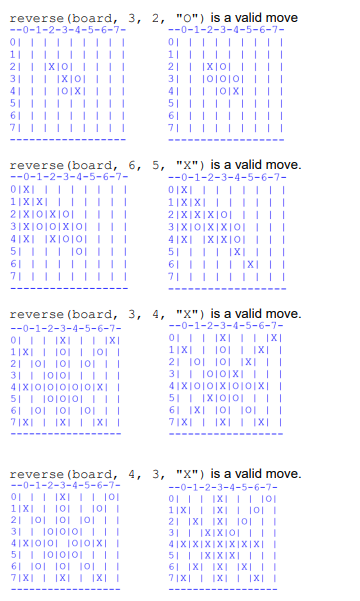
\includegraphics[width=0.5\paperwidth]{C:/Users/Admin/Desktop/Github/question_bank/LyX/static/img/9597-RVHS-2018-P1-Q4-1}
\par\end{center}

\subsection*{Evidence 20}

Program code of the iterative version of function \texttt{reverse}.
\hfill{}{[}5{]}

Program code of the recursive version of function \texttt{reverse}.
\hfill{}{[}5{]}

{[}SPLIT\_HERE{]}
\end{enumerate}

\end{document}
